\section{Scheduling Framework}
\label{Sec:Model}

% % \subsection{System Resources}
% % The system contains resources like compute nodes, main memory, burst buffer,
% % IO nodes and external storage.
% % In most system architecture, compute nodes are coupled with main memory.
% % Since storage capacity at most time is sufficient, we assume IO nodes are always available.
% % The schedule targets are compute node and burst buffer:
% % a system with $CN$ compute nodes and $BB$ GB of burst buffer.
% % BB are able to be shared by applications with any fractional amount.

%============XY==========

When users submit their jobs to burst buffer enabled systems, they can specify the 
demand of compute nodes, burst buffer and expected running time for each job.
The batch scheduler makes scheduling decision for each job based on its demand while trying to 
minimize overall job response time and maximize system throughput. 
However, jobs require for more than one resources could result in possible deadlock and starvation.\TODO{cite from OS}
In order to improve the overall resource utilization and system responsiveness, we propose
a fine granularity job model based on the possible usage cases of burst buffer.  
In our scheduling framework, 
the system resources that scheduler targets for making scheduling decision are
compute nodes and burst buffer.
Jobs' resource demand could change in different execution phases and the batch scheduler 
would make scheduling decision in each phase.


\subsection{Three-Phase Job Model}
% Users request the system to run their applications as jobs.
% We define $J = (job_1, job_2, \ldots, job_n)$ to be the set of all unfinished jobs in the system.
% To fully utilizing burst buffer, we divide jobs into 3 different phases.
% In the first phases, input data are staged in from IO nodes to burst buffer.
% We refer this phase as \textit{stage-in} phase.
% It is very easy for user to provide the amount of input data
% because they should already be available before application execution. 
% Then the job can run on the compute nodes after being scheduled;
% except reading data from burst buffer, there may be interaction between 
% computer node and burst buffer.
% These interactions are mainly due to fault tolerance reasons, like check-pointing.
% This phase is called \textit{running} phase.
% When computation is done, output data needs to be staged out to external PFS from memory,
% namely \textit{stage-out} phase.
% Burst buffer plays as an efficient IO broker for compute nodes,
% in replacing of traditional IO nodes.


%=============Xu======================
\begin{figure}[!htbp]
\centering
        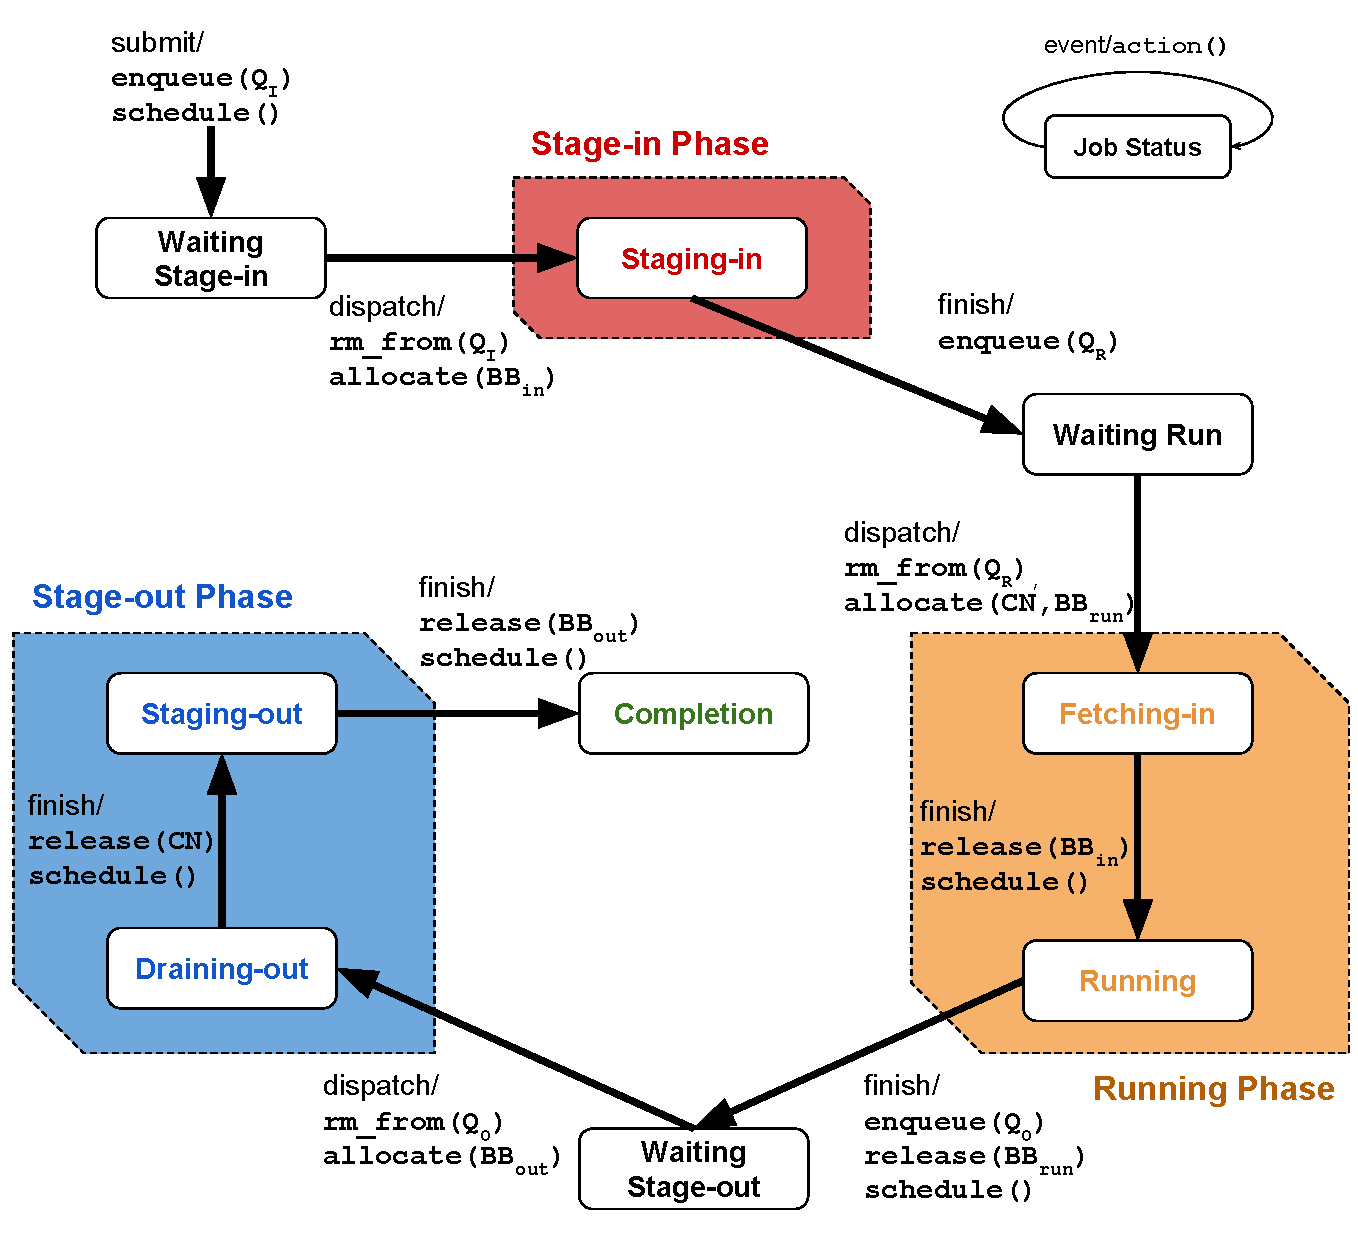
\includegraphics[width=3.6in]{3PhaseJobFSM}
        \caption{Event-driven BBsim scheduling model}
\label{Fig:JobFSM}
\end{figure}

With the help of burst buffer nodes,
jobs can pre-fetch data from external storage before running.
When jobs start running on compute nodes,
they could burst the checkpoint data to burst buffer at high speed.
Upton jobs completion, the output data can be staged out to burst buffer,
then drained out to external storage for the purpose of earlier releasing of compute node.
Therefore,
the job lifetime is divided up to three different phases in our scheduling framework.

\textbf{Stage-In}: After the job being submitted to the system,
         it needs to pre-fetch data, such as configuration files and input data,
         from IO nodes to burst buffer. We refer this phase as \textit{stage-in}.
         The only resource needed by the job in this phase is burst buffer.
         Users are encouraged to specify the amount of burst buffer required in the \textit{stage-in} phase.
         The job is ready to run when the data is pre-fetched into burst buffer.
 
\textbf{Running}: The scheduler will allocate the job with required
         number of compute nodes and the amount of burst buffer. 
         It will then dispatch the job to the system for running.
         This is referred as \textit{running} phase.
         During the running phase, there could be frequent data exchange
         between compute node and burst buffer.
         These interactions are mainly due to fault tolerance reasons, like check-pointing. 
 
\textbf{Stage-out}: When the job finishes computation and
         exit the \textit{running} phase, its output data needs to be drained out
         to external storage from the on-node memory. We refer this as \textit{stage-out} phase.
         The job can release its compute nodes when the output data is staged out
         into burst buffer at high speed. The burst buffer plays as an efficient
         IO broker for the compute nodes and drain the output data out to the external storage.

While burst buffer has been utilized during all three phases,
compute nodes are only required during the \textit{running} phase. 


\subsection{Three-Phase Resource Demand}
% Users typically provide their resource demand for their jobs.
% This is the most important information scheduler could get from the users.
% Therefore, each job is associated with a demand vector in the form of $(c, rt)$
% where $c$ is the number of needed compute node in running phase,
% $rt$ is the requested runtime user can provide to help scheduler make decisions.
% To be burst buffer aware, demand vector should be augmented
% with fields defining user's request for burst buffer capacity.
% We consider two possible ways to do so.
% Corresponding to the typical usage cases of burst buffer,
% user may provide a \textit{burst buffer triple} in the form of $(bb\_in, bb\_run, bb\_out)$,
% where $bb\_in$ is the volume of burst buffer user predicted for staging in data files,
% $bb\_run$ is the volume of burst buffer user preferred for checkpointing during running,
% $bb\_out$ is the volume of burst buffer needed to hold the resulting output data.
% A job that providing demand vector augmented with
% burst buffer triple is called a \textit{3-phase modeled job}.
% Alternatively, a lazy user may just use the $\max\{bb\_in, bb\_run, bb\_out\}$ at every stage.
% %We do not make any assumption about $bb\_run$ and $bb\_out$
% %because it is nontrivial to predict them, both for system scheduler and application owner.
% We refer this augmentation as
% \textit{1-phase modeled jobs} thereafter.

%=========XY===============
Jobs are submitted to system with specified resource demand. 
Each job is associated with a demand vector in the form of $(c, ert)$, 
where $c$ is the number of needed compute node in running phase,
$ert$ is the expected runtime. 
In a burst buffer enabled system, demand vector should be augmented
with fields defining user's request for burst buffer capacity.
We consider two possible ways that users provide burst buffer demand.
For the user with accurate speculation about his job's burst buffer demand in each phase,
he may provide a \textit{burst buffer triple} in the form of $(bb\_in, bb\_run, bb\_out)$,
where $bb\_in$ is the volume of burst buffer for staging in data files,
$bb\_run$ is for checkpointing during running,
$bb\_out$ is for staging out the output data.
% A job that providing demand vector augmented with
% burst buffer triple is called a \textit{3-phase modeled job}.
We will show that providing jobs burst buffer demand in the form of \textit{burst buffer triple} 
will yield great benefit in the following section.
Alternatively, a user may just use the $\max\{bb\_in, bb\_run, bb\_out\}$ 
as job's burst buffer demand in the whole lifetime. 
% We refer this augmentation as
% \textit{1-phase modeled jobs} thereafter.

% The tightly coupling between processing cores and memory makes 3-phase model
% more complicated than it appears in terms of resource releasing.
% For a job at the stage-in phase, compute nodes is not allocated to it yet
% but that will not effect staging in data.
% When scheduler allocate compute nodes (coupled with memory) to a job,
% these nodes are exclusively used by this job.
% The first thing to do in running phase is fetching in data from burst buffer to memory,
% which is not available until compute nodes is allocated to job.
% We refer this sub-phase as \textit{fectch-in} phase.
% $bb\_in$ will be hold by job until \textit{fetch-in} phase finished.
% Even if the computation is done when job exit \textit{running phase},
% compute nodes cannot be released until job enters \textit{stage-out} phase 
% \textbf{and} output data are drained out to burst buffer from memory,
% referred as \textit{drain-out} phase.
% However, $bb\_run$ can be immediately reclaimed at the end of \textit{running phase}.
% Once \textit{drain-out} phase is done,
% compute nodes become available for jobs waiting to be run
% because staging output data out to IO node is the business of burst buffer nodes,
% sometimes with the help from traditional IO nodes.
% Burst buffer nodes used for caching output data can thus be put back for reuse
% when \textit{stage-out} phase, as well as the entire lifetime of job, concludes.


%==========XY=====================
The resource releasing for the 3-phase modeled jobs is nontrivial. 
For a job at \textit{stage-in} phase, compute nodes is not allocated to it yet. 
The job can stage in data from external storage to burst buffer without the involvement of compute nodes.
When scheduler allocates compute nodes to the job, the job enters the \textit{running} phase 
and starts to read the pre-fetched data from burst buffer into the main memory, 
$bb\_in$ will be released after all the data are moved into main memory. 
When the job finishes computation and exits \textit{running} phase, 
$bb\_run$ are released while compute nodes are still hold by the job. 
The compute nodes will be released after all the output data are moved into $bb\_out$ from main memory.
The job at \textit{stage-out} phase only holds $bb\_out$ burst buffer. 
Once all the output data are drained out to the external storage,  
$bb\_out$ is released.


\begin{table}[!htbp] 
        \renewcommand{\arraystretch}{1.3}
        \caption{Summary of Symbols}
        \label{Tab:Symbols}
        \centering
        \begin{tabular}{l|l}
                \hline
                $CN$ & number of total compute nodes \\
                $BB$ & amount of total burst buffer nodes \\
                $CN_{available}$ & number of available compute nodes \\
                $BB_{available}$ & amount of available burst buffer nodes \\
                $c_i$ & compute node demand of $job_i$ \\
                $bb\_in_i$ & burst buffer demand of $job_i$ at \textit{stage-in} phase \\
                $bb\_run_i$ & burst buffer demand of $job_i$ at \textit{running} phase \\
                $bb\_out_i$ & burst buffer demand of $job_i$ at \textit{stage-out} phase \\
%                 $rt_i$ & running time of $job_i$ \\
                $ert_i$ & estimated or expected running time of $job_i$ \\
                $Q_I, Q_R, Q_O$ & queues for \textit{stage-in, running, stage-out} phase \\
                $J_{Q_I}, J_{Q_R}, J_{Q_O}$ & set of jobs in corresponding queue \\
                $S$ & set of jobs selected by scheduler \\
                $v_i$ & value of $job_i \in J_{Q_R}$ defined by Equation~\ref{Equ:DefValue}\\
                $dp(\cdot)$ & memo used in dynamic programming \\
%                 $TS_{s\_x}$ & event timestamps of starting phase $x$ in simulation \\
%                 $TS_{f\_x}$ & event timestamps of finishing phase $x$ in simulation \\
                \hline
        \end{tabular}
\end{table}

